\chapter{METHODOLOGY}
\section{Methodology}
This seminar report is more focus on feature extraction of Nepali news dataset for the text classification task. Additionally, web scraping process is used for the data collection. The figure \ref{fig:Overall} illustrate the step carry out in this seminar report.
\begin{figure}[H]
	\centering 
	\vspace{10pt}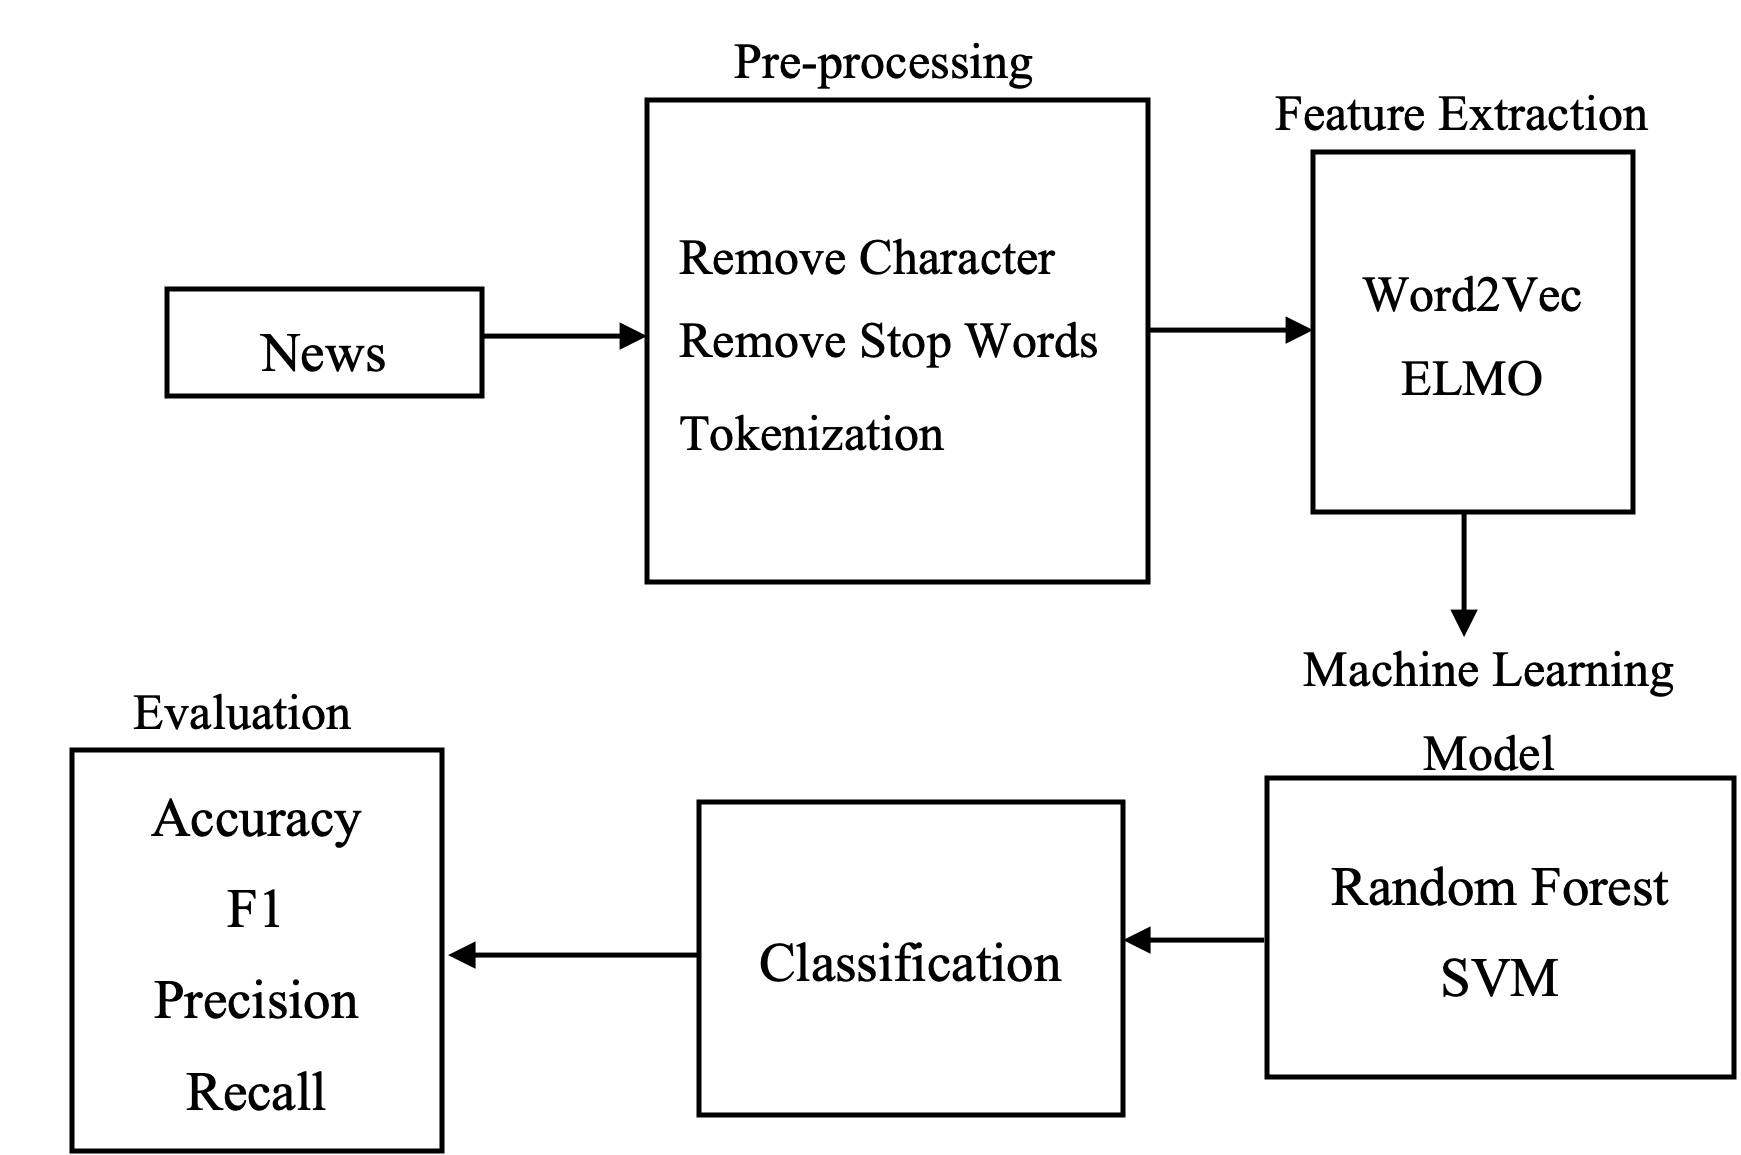
\includegraphics[width=10cm]{images/methodology.png}
	\caption{Overall Process} 
	\label{fig:Overall}
\end{figure}
\section{Dataset Discription}
There are total of 5145 news articles which are scraped from www.ekantipur.com, in four different categories. Categories are Health, National, Opinion, Business. The detail of the dataset is given in the table \ref{table:Dataset}. 
\begin{center}
\begin{table}
\caption{Dataset Description}
\label{table:Dataset}
\centering
\begin{tabular}{ |p{3cm}||p{3cm}|p{3cm}|p{3cm}|  }
 \hline
 Category& Total Data \\
 \hline
 Health   & 1029    \\
 Opinion&   1029  \\
 National &1029\\
 News &1029 \\
 \hline
\end{tabular}
\end{table}
\end{center}
\section{Data Preprocessing}
This step cleans the document by removing HTML tags and noisy characters present in the document, by using different python libraries such as NLTK and regular expression.
\subsection{Remove Special Characters}
Special characters play the negative role in the machine learning algorithm. So, they are removed by using the regular expression library available in the python programming language.
\subsection{Remove Stop Words}
A stop words is a commonly used word that a search engine has been programmed to ignore, both when indexing entries for searching and retrieving them as the result of a search query. Additionally, these data may not play the significant role for the result, so here remove them easily by storing a list of words by considering to be stop words. NLTK (Natural Language Toolkit) in python has a list of stop words stored in 16 different languages.
\subsection{Tokenization}
Tokenization describes splitting paragraphs into sentences, or sentences into individual words. For the former Sentence Boundary Disambiguation (SBD) can be applied to create a list of individual sentences. This relies on a pre-trained, language specific algorithms like the Punkt Models from NLTK. Sentences can be split into individual words and punctuation through a similar process. This seminar report uses tokenization in preprocessing task by using Punkt Models from NLTK.
\section{Feature Extraction}
\subsection{Word2Vec}
Word2Vec is a statistical method for efficiently learning a standalone word embedding from a text corpus. It was developed by Tomas Mikolov \cite{mikolov2013efficient} as a response to make the neural-network-based training of the embedding more efficient then has become the de facto standard for developing pre-trained word embedding. Word2Vec is a method to construct such  embedding. It can be obtained using two methods: Skip Gram and CBOW. The figure \ref{fig:CBOW} show the architecture of CBOW
\begin{figure}[H]
	\centering 
	\vspace{20pt}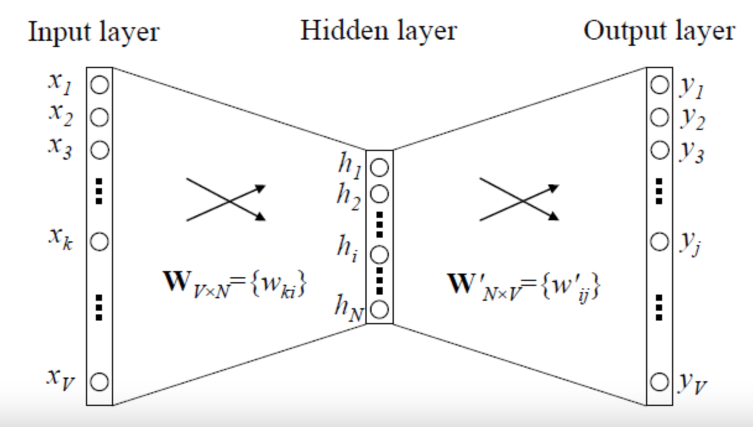
\includegraphics[width=10cm]{images/Word2Vec.png}
	\caption{The CBOW architecture predicts the current word} 
	\label{fig:CBOW}
\end{figure}
Word representations in Word2Vec are taken from a simple neural network, which consists of:
\begin{itemize}
  \item {An input layer}
  \item {A projection layer}
  \item {One hidden layer}
  \item{One output layer}
\end{itemize}
The input is the one hot encoded representation of a word, and the projection layer has dimensionality N*D, while the hidden layer is typically 300 units and learns dense representation. Additionally, the hidden layer has no activation function.
\subsection{ELMo}
The ELMo is a novel way to represent words in vectors or embedding. It was developed by Sarzynska-Wawer, \cite{sarzynska2021detecting}, and these word embeddings are helpful in achieving state-of-the-art (SOTA) results in several NLP tasks such as text classification, machine translation and sentiment analysis.
Unlike most widely used word embedding, ELMo word representations are functions of the entire input sentence. They are computed on top of the two-layer biLMs with character convolution, as a liner function of the internal network state. This setup allows to do semi-supervised learning, where the biLM is pretrained at a large scale and easily incorporated into a wide range of existing NLP architectures. The ELMo architecture is shown in the figure \ref{fig:ELMo}.
\begin{figure}[H] 
	\centering 
	\vspace{20pt}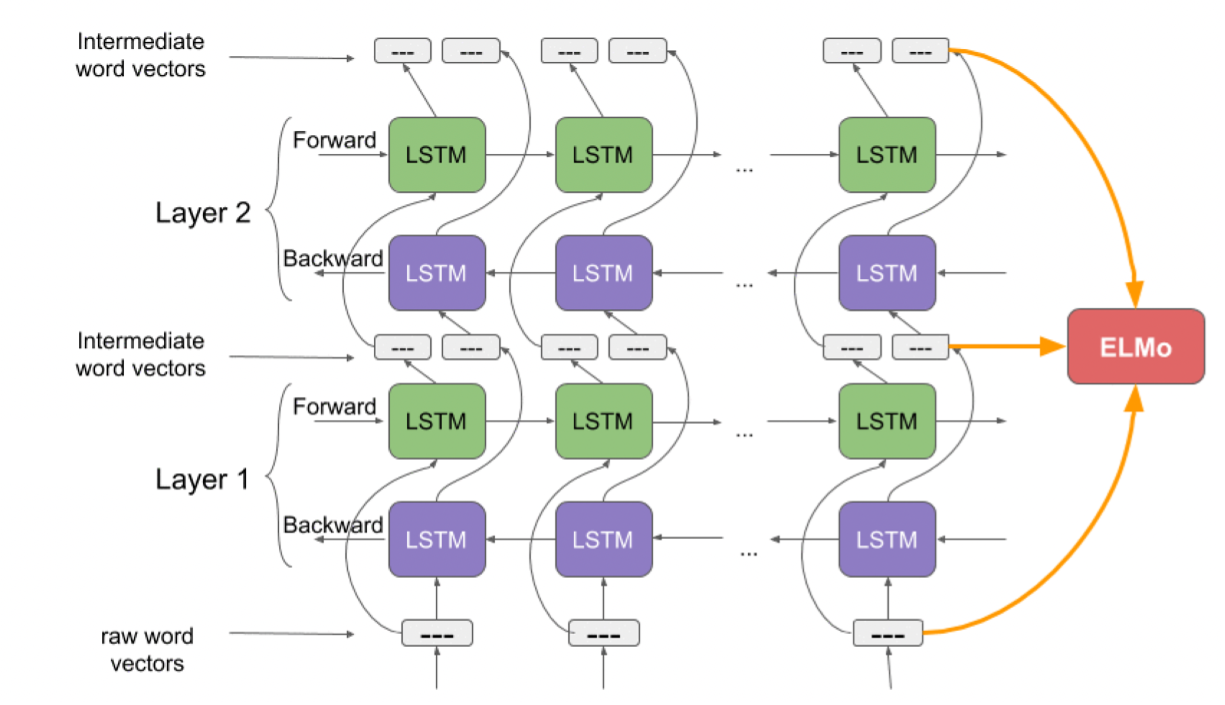
\includegraphics[width=10cm]{images/ELMO.png}
	\caption{Architecture of ELMo}
	\label{fig:ELMo} 
\end{figure}
\section{Machine Learning Model}
\subsection{SVM}
The SVM algorithm is a ‘simple’ linear classification/regression algorithm. It tries to find a hyper plane which separates the data in two classes as optimally as possible. Here as optimally as possible means that as many points as possible of label A should be separated to one side of the hyper plane and as points of label B to the other side, while maximizing the distance of each point to this hyper plane. The hyperplane used in the support vector machine is shown in the figure \ref{fig: SVM_hperplane}.\\
\begin{figure}[H] 
	\centering 
	\vspace{20pt}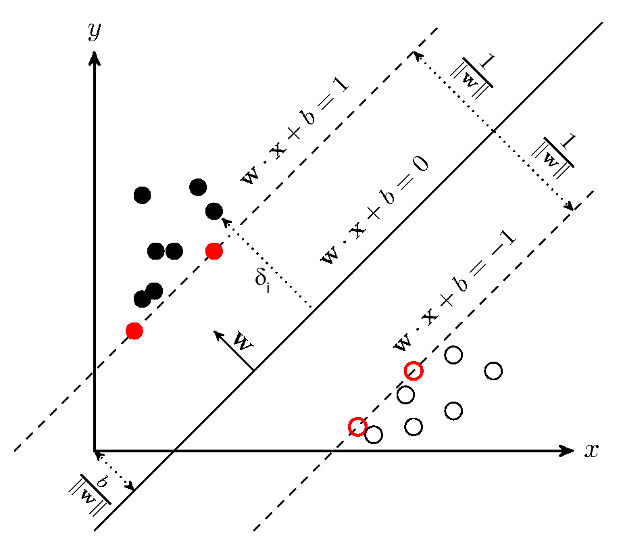
\includegraphics[width=10cm]{images/SVM.png}
	\caption{Support Vector machine hyper plane} 
	\label{fig: SVM_hperplane}
\end{figure}
\textbf{Steps involved in SVM algorithm:}\\
Step 1. Read the training data set. \\
Step 2. Prepared the pattern matrix.\\ 
Step 3. Select kernel function to use. \\
Step 4. Select parameter of the kernel function and value of c \\
Step 5. Execute the training algorithm
\subsection{Random Forest}
Random forest is a supervised machine learning algorithm that is used widely in classificati-on and regression problems. It builds decision tree on different samples and takes their majority vote for classification and average in case of regression. Additionally, one of the most important features of the random forest algorithm is that it can handle the data set containing continuous variable as in the case of regression and categorical variables as in the case of classification.\\
Random forest algorithm is worked on the bagging principal. It is also known as Bootstrap Aggregation is the ensemble technique used by random forest. Bagging chooses random sample from the dataset. Hence each model is generated from the samples provided by the original data with replacement known as row sampling. Additionally, each model is trained independently which generate results. The final output is based on majority voting after combining the results of all models. All in all, the step which involves combining all the results and generating output based on majority voting is known as aggregation. The overall structure of the random forest algorithm is depicted in the figure \ref{fig:random_forest}.\\
\begin{figure}[H] 
	\centering 
	\vspace{20pt}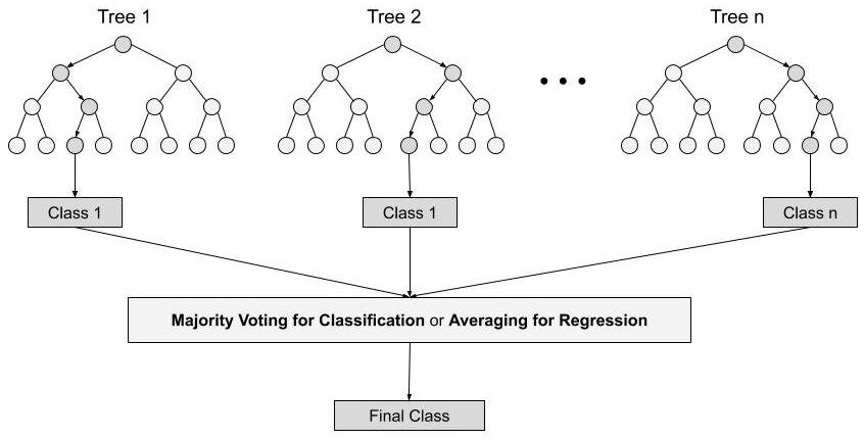
\includegraphics[width=10cm]{images/randomforest.jpg}
	\caption{Random Forest Classifier}
	\label{fig:random_forest} 
\end{figure}
\textbf{Steps involved in random forest algorithm:}\\
Step1: n number of random news are taken from the given dataset.\\
Step2: individual decision trees are constructed for each taken sample news.\\
Step3: each decision tree will generate an output.\\
Step4: final output is considered based on majority voting or average for the news classification
\section{Evaluation Techniques}
\subsection{Accuracy}
In news classification, Accuracy Score is the ratio of correctly predict news classes to the total number of input data points. It can be calculated by using following formula. \
\[ 
 Accuracy=\frac{(TP+TN)}{(TP+FN+TN+FP)} 
\]
Where, \\
TP is the number of True Positive instance\\
FN is the number of False Negative instance\\
FP is the number of False Positive instance\\
TN is the number of True Negative instance
\subsection{Precision}
Precision is the ratio of number of True Positive to the total number of Predicted Positive . It measures out of the total predicted positive, how many are actually positive. All in all, precision score is calculated by using following formula.\
\[ 
 Precision Score=\frac{TP}{(FP+TP)} 
\]
Where,\\
TP is the number of true positive instance\\
FP is the number of false positive instance
\subsection{Recall}
Recall is the ratio of number of True Positive to the total number of Actual Positive. It measures out of the total actual positive, how many are predicted as True Positive, and it can be calculated by using following formula.\
\[ 
 Recall Score=\frac{TP}{(FN+TP)} 
\]
Where,\\
TP is the number of true positive instance.\\
FN is the number of false-negative instance.
\subsection{F1 Score}
It is an important evaluation matric for binary classification that combines Precision and Recall. F1 score is the harmonic mean of precision and recall, whcih is obtained by the following calculation.\
\[ 
 F1 Score=2*\frac{Precision Score*Recall Score}{(Precision Score+Recall Score)} 
\]